% !TeX spellcheck = en_GB
\section{Simulations Experiments}
\subsection{Scenario Calibration}
In order to calibrate the simulator parameters, the following range of values were used:
\begin{itemize}
	\item \textbf{Number of Couples Tx-Rx (N)}: [5, 30]
	\item \textbf{Number of Channels (C)} : [6, 100] (Resource Blocks in LTE for different Frequencies)
	\item \textbf{Mean Inter-arrival Time ($\frac{1}{\lambda}$)}: [125ms, 500ms] (a study was performed in order to choose the mean inter-arrival time that allow us to have meaningful data)   
	\item \textbf{Time-slot duration ($T_{slot}$)}: 5 ms
	\item \textbf{Send Probability (p)}: [0.1, 0.5] 
\end{itemize}

\subsection{Calibration of Warm-Up Period and Simulation duration}
For calibrating the warm-up different simulation were made (with the factors range in the latter paragraph). After various test is clear that the KPI that impacts heavily in the choose of the warmup time is the \textit{Response Time}. We can see the study about the response time in figure \ref{img: warmUp}.
%The worst case in terms of convergence time was encountered with the \textbf{mean throughput} with N = 5, C = 6, $\dfrac{1}{\lambda}$ = 500ms, p = 0.5:
\begin{figure}[H]
	\centering
	\includegraphics[width=\textwidth]{img/warmup.png}
	\caption{Worst Case Warm-up Response Time}
	\label {img: warmUp}
\end{figure}  
%With the \textbf{mean response time} the worst case is the following with N = 5, C = 100, $\dfrac{1}{\lambda}$ = 25ms, p = 0.5:

\noindent\textbf{A warm-up period of 250s was chosen}.\\
For what concerns the simulation duration was made a trade-off between the memory consumption for storing data and the length of the simulation itself. This was done because there are not stochastic elements in the model (like a particular error probability with a low percentage) that will need a particular amount of time to be shown. Obviously the duration has to be greater than the warm-up duration. All things considered, \textbf{a simulation-duration of 5000s was chosen}.

\subsection{Design of Experiments}
\subsubsection{Factorial Analysis $r2^k$ on Throughput}
In order to analyse the contribution of the factors on the throughput performance, we perform a $r2^k$ analysis with $r=5$ and $k=4$ (so we perform $5*2^4 = 80$ experiments). We take into account the following factors:
\begin{itemize}
	\item Number of Couples Tx-Rx: [5, 30] \textbf{(A)}
	\item Number of Channels C : [6, 100] \textbf{(B)}
	\item Send Probability p: [0.1, 0.5] \textbf{(C)}
	\item Mean Inter-arrival Time: [125ms, 500ms] \textbf{(D)}    
\end{itemize}

\noindent The first step is to check the hypothesis, in particular we have to control that the residuals are normal and that its standard deviation is constant (a.k.a. homoskedasticity). For what concerns the normal hypothesis it's possible to see (Figure \ref{img: qqplot_throughput}) that the QQ plot of residuals vs normal show a linear tendency and so the hypothesis is verified.

\noindent For the homoskedasticity, we have a QQ plot residuals vs predicted response and we can see (Figure \ref{img: homoskedasticity_throughput}) that indeed there is a trend, however the errors (y axis) are two order of magnitude below the predicted response (x axis) and so we can ignore trends and state that the homoskedasticity hypothesis is respected.

\begin{figure}[H]
	\centering
	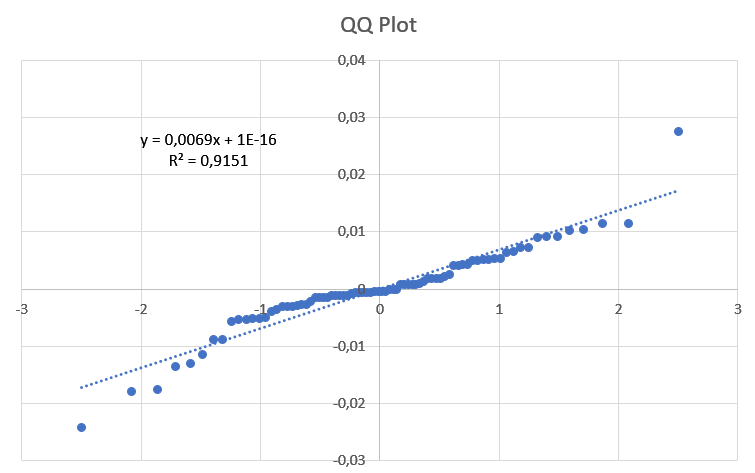
\includegraphics[width=0.8\textwidth]{img/QQplot_2kr_throughput.png}
	\caption{QQ Plot for testing the normal hypothesis}
	\label {img: qqplot_throughput}
\end{figure}

\begin{figure}[H]
	\centering
	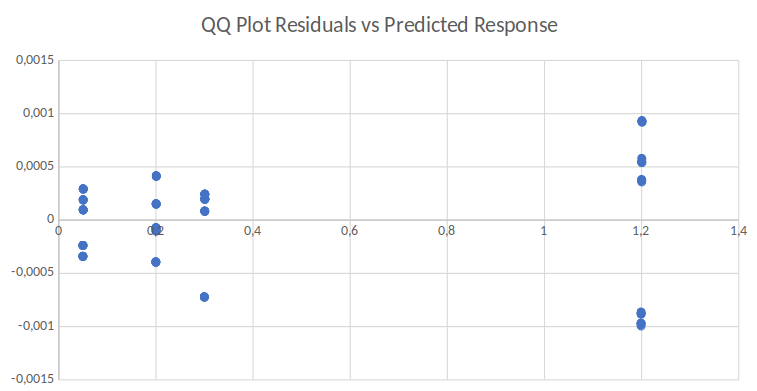
\includegraphics[width=0.8\textwidth]{img/homoskedasticity_2kr_throughput.png}
	\caption{QQ Plot for testing homoskedasticity}
	\label {img: homoskedasticity_throughput}
\end{figure}

\noindent Now we can analyse the obtained results. The most relevant ones are the one in the following list, the other factors have an impact on the variability that is very low, ($<<1\%$) and so they are non relevant:

\begin{itemize}
	\item \textbf{Number of Couples}
	
	\noindent It has a positive impact on throughput, in particular $qi = [0,312532; 0,312537]$\footnote{This and the following are 95\% confidence interval} and it accounts for the 48,44\% of the variability. This means that the higher the number of couples the higher the throughput. In fact with more transmitters we have more packets and so we have an higher throughput.
	 
	\item \textbf{Mean Inter-Arrival Time}
	
	\noindent It has a negative impact: $qi = [-0,262444; -0,262439]$ and it accounts for the 34,15\% of the variability. Thus we can say that the higher the mean inter-arrival time, the lower the throughput. This happens due to the fact that when we increase the mean inter-arrival time it's more likely that a transmitter have an empty buffer and so it has no packets to transmit, then the throughput decreases. 
	
	\item \textbf{Jointly Effect of Number of Couples and Mean Inter-Arrival Time}
	
	\noindent The jointly effect of the above factors accounts for the 17,39\% of the variability and it has a negative impact ($qi = [-0,187301; -0,187296]$). This because the effect of the mean inter-arrival time is greater with respect to the one of the number of couples, so if both increase then the throughput decreases. Indeed, if we have an higher number of transmitters, but we have the most of them which have an empty buffer (due to the previously explained phenomenon caused by the increasing of the mean inter-arrival time), then the throughput decreases because there are too few packets to transmit.
\end{itemize}

\subsubsection{Factorial Analysis $r2^k$ on Response Time}
Now let analyse the contribution of factors on the other KPI, the response time. Also in this case, as the previously, we perform a $r2^k$ analysis with $r=5$ and $k=4$ and so 80 experiments in total. The factors are the same of the previously analysis.

\noindent We can see the plots to check the hypothesis in figure \ref{img: qqplot_responsetime} (for what concerns the normal hp) and in figure \ref{img: homoskedasticity_responsetime} (for what concerns the homoskedasticity).

\begin{figure}[H]
	\centering
	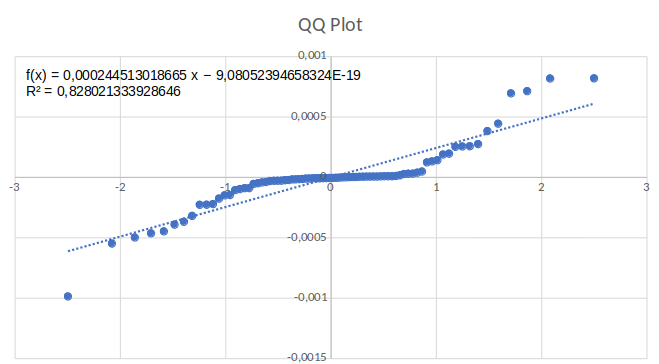
\includegraphics[width=0.8\textwidth]{img/qqplot_2kr_responsetime.png}
	\caption{QQ Plot for testing the normal hypothesis}
	\label {img: qqplot_responsetime}
\end{figure}

\begin{figure}[H]
	\centering
	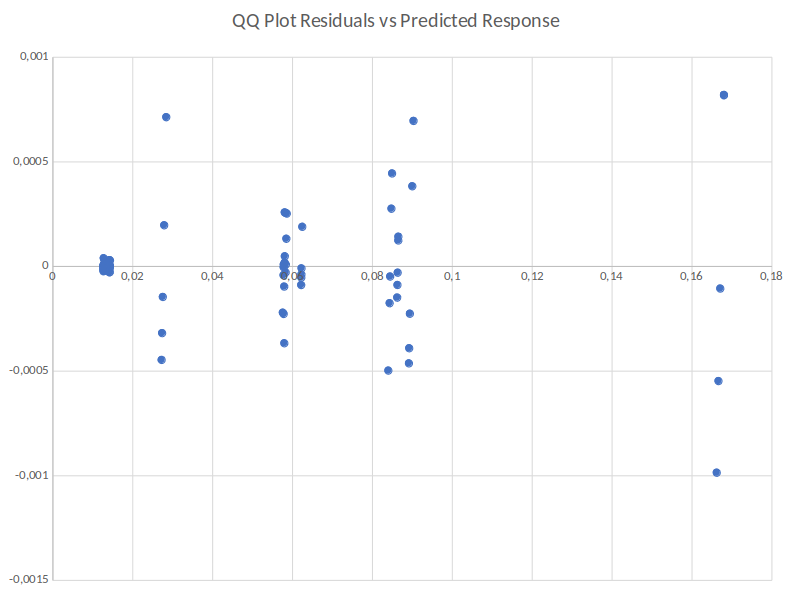
\includegraphics[width=0.8\textwidth]{img/homoskedasticity_2kr_responsetime.png}
	\caption{QQ Plot for testing homoskedasticity}
	\label {img: homoskedasticity_responsetime}
\end{figure}

\noindent The plot about the normal hp is obtained through a logarithmic transformation and it shows an approximating linear trend. Instead for the homoskedasticity we can see that there is a trend but the errors are at least one order of magnitude below the predicted response, and so also this hypothesis is verified.

\noindent The most relevant contributions are the ones explained in the following lists, the others one have an impact in the variability that is negligible w.r.t. the following ones: 

\begin{itemize}
	\item \textbf{Send Probability}
	
	\noindent It has a negative impact on the response time, in particular $qi = [-0,033928; -0,033926]$ and it accounts for the 65,67\% of the variability. This means that the higher the send probability the lower the response time. In fact with an high send probability it's more likely that a packet will sent (both in the case of first transmission and in the case of retransmission because of collision) and so it doesn't remain in the transmitter queue increasing its response.  
	
	\item \textbf{Mean Inter-Arrival Time}
	
	\noindent It has a negative impact: $qi = [-0,012955; -0,012954]$ and it accounts for the 9,57\% of the variability. Thus we can say that the higher the mean inter-arrival time, the lower the response time. This happens due to the fact that when we increase the mean inter-arrival time it's more likely that transmitters send few packets in a slot time and so the probability of having collisions, and so the necessity of retransmitting a packet, is lesser. Moreover even if a collision occurs with an higher mean inter-arrival time there are not several packets in the transmitter queue and so the response time decreases. 
\end{itemize}

\newpage
\subsubsection{$r2^k$ Overall Results}
In the table \ref{tab: 2kr_results} we can see the results obtained through the $r2^k$ analysis.
\begin{table}[H]
	\centering
	\begin{tabular}{|c|c|c|c|c|}
		\hline
		\textbf{} & \multicolumn{2}{c|}{\textit{\textbf{Throughput}}} & \multicolumn{2}{c|}{\textit{\textbf{Response Time}}} \\ \hline
		Factors   & qi          & Impact on Variability (\%)          & qi            & Impact on Variability (\%)           \\ \hline
		A    &  & 48,44 \%    & \textbf{} & 2,18\%  \\ \hline
		B    &  & 9,35 x $10^{-11}$ \% & \textbf{} & 2,57 \%  \\ \hline
		C    &  & 2,23 x $10^{-10}$ \% & \textbf{} & 65,67 \% \\ \hline
		D    &  & 34,15\%    & \textbf{} & 9,57\%  \\ \hline
		AB   &  & 1,03 x $10^{-11}$ \% & \textbf{} & 1,96 \%  \\ \hline
		AC   &  & 4,08 x $10^{-10}$ \% & \textbf{} & 1,04 \%  \\ \hline
		AD   &  & 17,39 \%    & \textbf{} & 1,71\%  \\ \hline
		BC   &  & 1,58 x $10^{-10}$ & \textbf{} & 1,21 \%  \\ \hline
		BD   &  & 9,35 x $10^{-11}$ \% & \textbf{} & 1,99 \%  \\ \hline
		CD   &  & 1,93 x $10^{-11}$ \% & \textbf{} & 6,84 \%  \\ \hline
		ABC  &  & 1,17 x $10^{-10}$ \% & \textbf{} & 0,93 \%  \\ \hline
		ABD  &  & 1,03 x $10^{-11}$ \% & \textbf{} & 1,56 \%  \\ \hline
		ACD  &  & 3,62 x $10^{-10}$ \% & \textbf{} & 0,88 \%  \\ \hline
		BCD  &  & 2,23 x $10^{-10}$ \% & \textbf{} & 1,02 \%  \\ \hline
		ABCD &  & 1,17 x $10^{-10}$ \% & \textbf{} & 0,80 \%  \\ \hline
	\end{tabular}
	\caption{Results of $r2^k$ analysis for Throughput and for Response Time}
	\label{tab: 2kr_results}
\end{table}
																
\subsection{Result Analysis}
Our objective is (as we said at the beginning of the report) the \textit{Assessment of the Effectiveness of the Slotted Random-Access Network Protocol}. In order to do so we choose the mean response time and the mean throughput as Key Performance Indexes. For each KPI we set 2 scenarios: one for low traffic condition and the other one for high traffic condition. For each factor variation of each scenario of each KPI we perform 35 repetitions in order to obtain meaningful and statistically valid data. Data are computed with a confidence level of 95\% (to small to be seen) .Thanks to the analysis performed on this two scenarios and studying the evolution of the KPIs in them, we are able to reach our aim and give some final conclutions on the network protocol. 

\subsubsection{Throughput}
For what concerns the throughput we set these two scenarios:
\begin{enumerate}
	\item \textit{High Traffic Scenario}
	
	N = 30, C = 6, Send Probability = 0.1
	\item \textit{Low Traffic Scenario}
	
	N = 5, C = 100, Send Probability = 0.1
\end{enumerate}

\noindent In both scenarios we vary the mean inter-arrival time from 125 ms to 500 ms with a step of 75 ms. In fact as we seen in the $r2^k$ analysis it is the most relevant factor for the throughput. 

\noindent We can see the results obtained in the outlined scenarios when the mean inter-arrival time grows from 125 ms to 500 ms in figure \ref{img: insight1_throughput}.

\begin{figure}[H]
	\centering
	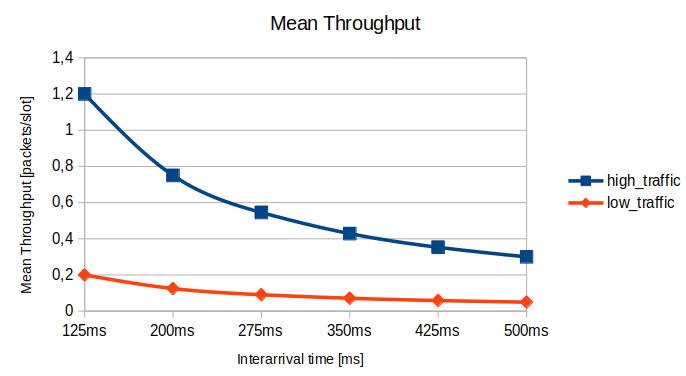
\includegraphics[width=\textwidth]{img/insight1_throughput.png}
	\caption{Insight 1}
	\label{img: insight1_throughput}
\end{figure}

\noindent From the plot we can state that the throughput is higher in the high traffic scenario, because the more the traffic the more the packets. We can also see that the best results is obtained with the lower mean inter-arrival time, this because we have to consider the time slot duration that is 5 ms and it is a lot smaller than the mean inter-arrival time: if the mean inter-arrival time increases, then there are slots where no packets are transmitted (because transmitters have no packets in the queue) and this affect the mean throughput and this is the reason why the throughput decreases with the increase of the mean inter-arrival time. So the latter is another validation of what we obtain from the $r2^k$ analysis. So at the end we can say that the throughput depends mainly from the traffic and from the mean inter-arrival time, this is good because this means that the effect of collisions doesn't not affect so much the overall performance of the network protocol. In fact in the high traffic condition there are more collisions w.r.t. to the scenario with low traffic, but nevertheless the throughput it is not affected by this.

\noindent Now let analyse the fairness of the network protocol for what regards the throughput. It's possible to see the Lorenz Curve for both scenarios in figure \ref{} and in figure \ref{}.

\subsubsection{Response Time}
For what concerns the response time we set these two scenarios:
\begin{enumerate}
	\item \textit{High Traffic Scenario}
	
	N = 30, C = 6, Mean Inter-Arrival Time = 125 ms
	\item \textit{Low Traffic Scenario}
	
	N = 5, C = 100, Mean Inter-Arrival Time = 125 ms
\end{enumerate}

\noindent In both scenarios we vary the send probability from 0.1 to 0.5 with a step of 0.1, in fact for the response time the latter is the most relevant factor (as we seen in the $r2^k$ analysis) and so it is the only that if changes causes a big difference.

\noindent The results obtained in the previously explained scenario when the send probability (p) varies from 0.1 to 0.5 is shown in figure \ref{img: insight1_respTime}.
\begin{figure}[H]
	\centering
	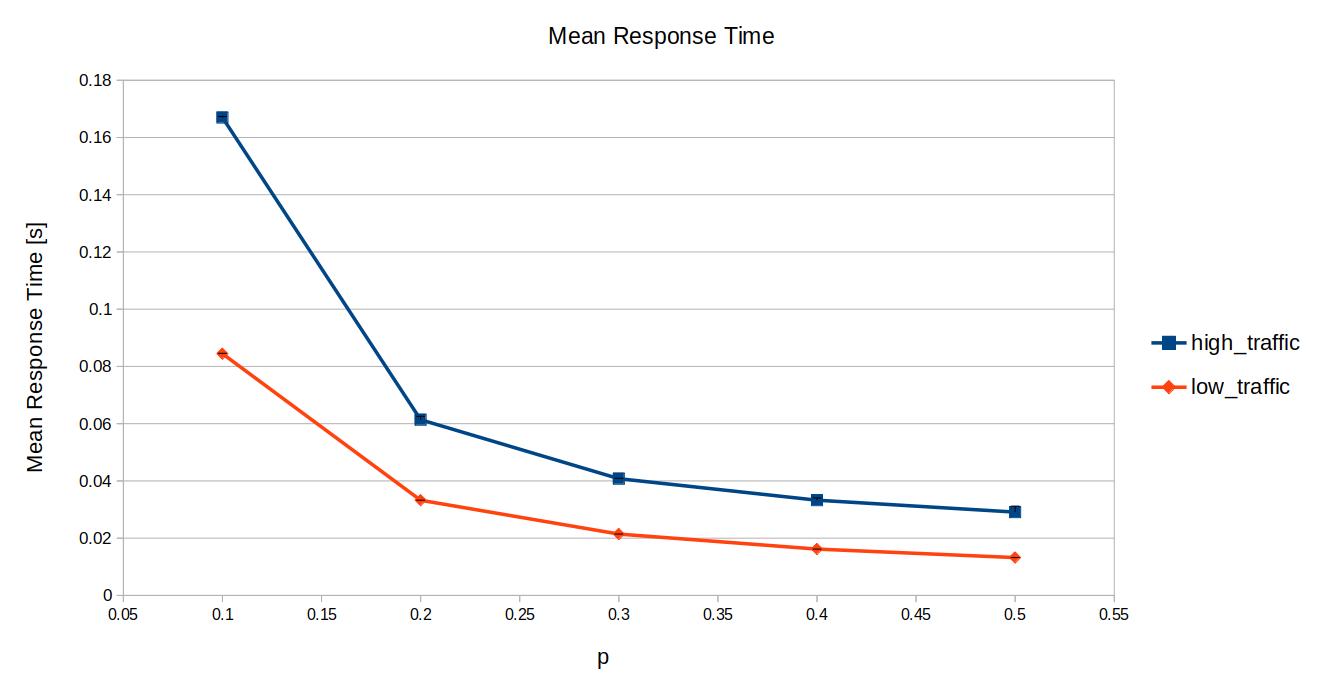
\includegraphics[width=\textwidth]{img/MeanResponseTimeInsight.png}
	\caption{Insight 1}
	\label{img: insight1_respTime}
\end{figure}

\noindent From the figure we can infer that in the high traffic scenario the response time is higher than the low traffic scenario, this is something normal. Then we can also say that the mean response time decreases with the increasing of the send probability (as we expected from the $r2^k$ analysis) and that the difference between the two scenarios are lower when p increases. The greater value is about 0.17 seconds that are equal to 170 ms which is not a good response time but it is acceptable one and it is a response time which can be experimented also by other network protocols.

\noindent Now let focus on the fairness of the protocol as regards the response time. We can see Lorenz Curve for the high traffic scenario in figure \ref{img: insight2_respTime} and Lorenz Curve for the low traffic scenario in figure \ref{img: insight3_respTime}.

\begin{figure}[H]
	\centering
	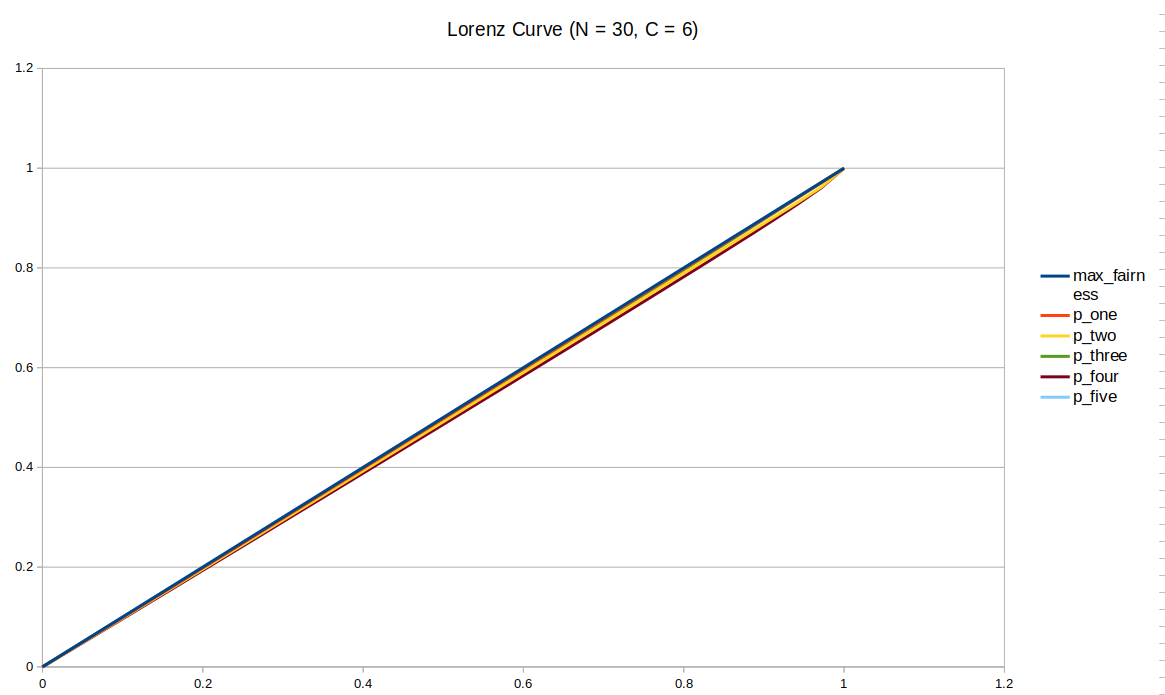
\includegraphics[width=\textwidth]{img/LorenzHighTraffic.png}
	\caption{Insight 2}
	\label{img: insight2_respTime}
\end{figure}
\begin{figure}[H]
	\centering
	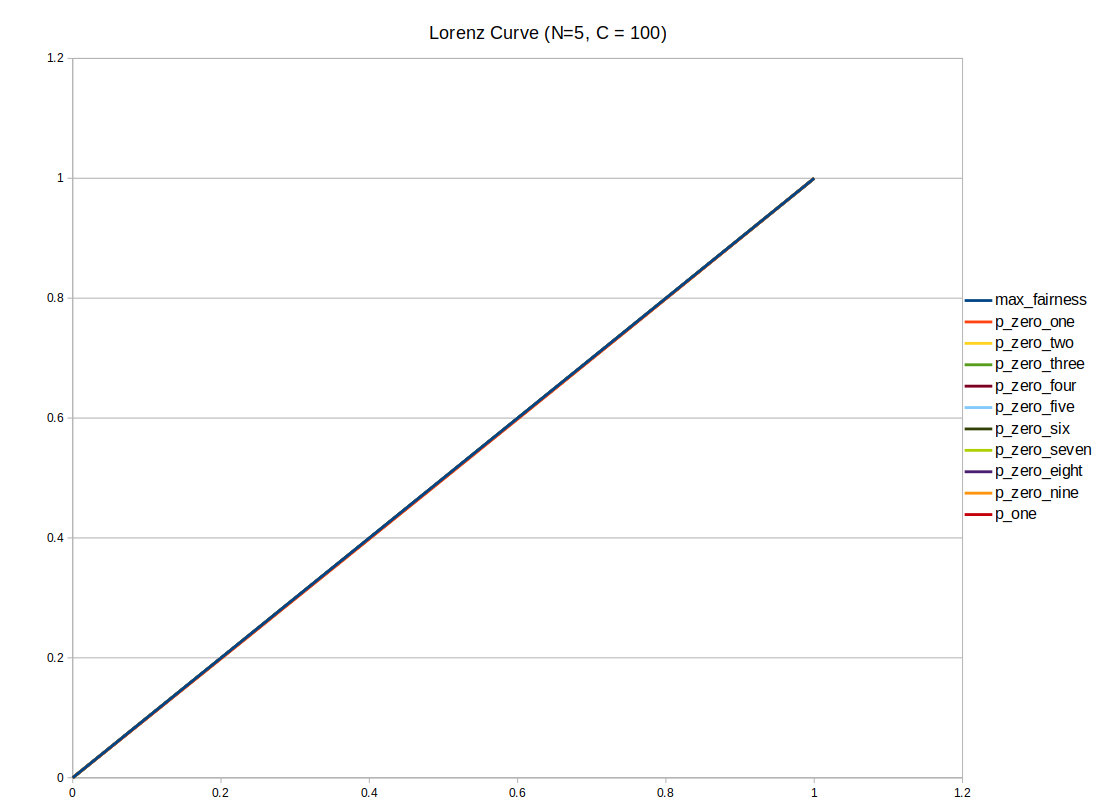
\includegraphics[width=\textwidth]{img/LorenzLowTraffic.png}
	\caption{Insight 3}
	\label{img: insight3_respTime}
\end{figure}

\noindent We can see that in both cases the curve related to the simulation scenarios are very close to the line of maximum fairness (in the case of low traffic they are overlapping). So we can say that the network protocol is absolutely fair for what regards the response time, whatsoever be the traffic condition.

